%!TEX program = xelatex
\documentclass[cn,hazy,pku,12pt,normal,math=newtx,cite=super]{elegantnote}
\title{蔗糖的转化}

\author{刘松瑞 \quad 2100011819 \\ 组号:24 \quad 组内编号:5}
\institute{化学与分子工程学院}

\expdate{\zhdate{2023/10/11}}
\temperature{20.1 \si{^{\circ}C}}
\pressure{101.38 \si{kPa}}

\usepackage{gensymb}
\usepackage{array}
\usepackage{subfigure}
\usepackage[fontset=windows]{ctex}
\usepackage{graphicx}
\usepackage{float}
\usepackage{caption}
\usepackage{multirow}
%\usepackage{subfig}
%\usepackage{float}
\begin{document}

\maketitle

\keywords{化学动力学\quad反应级数\quad半衰期\quad旋光仪}

\abstracts{
    本实验测量了蔗糖转化反应中蔗糖的反应级数,表观速率常数等化学反应动力学性质,并研究了对氢离子浓度的
    反应级数。实验方法上借助对旋光度的测量,间接地测量溶液中蔗糖浓度的变化,并以
    此来计算该反应的化学反应动力学常数。通过对不同氢离子浓度下的蔗糖转化反应,可以得到对蔗糖的反应级数为一级反应,对氢离子为二级反应。
}

\newpage


\section{引言}

\subsection{实验目的、原理和方法}

实验目的、原理和方法详见预习报告图~\ref{1} 与图 \ref{b} 。

\begin{figure}[htbp]
    \centering
    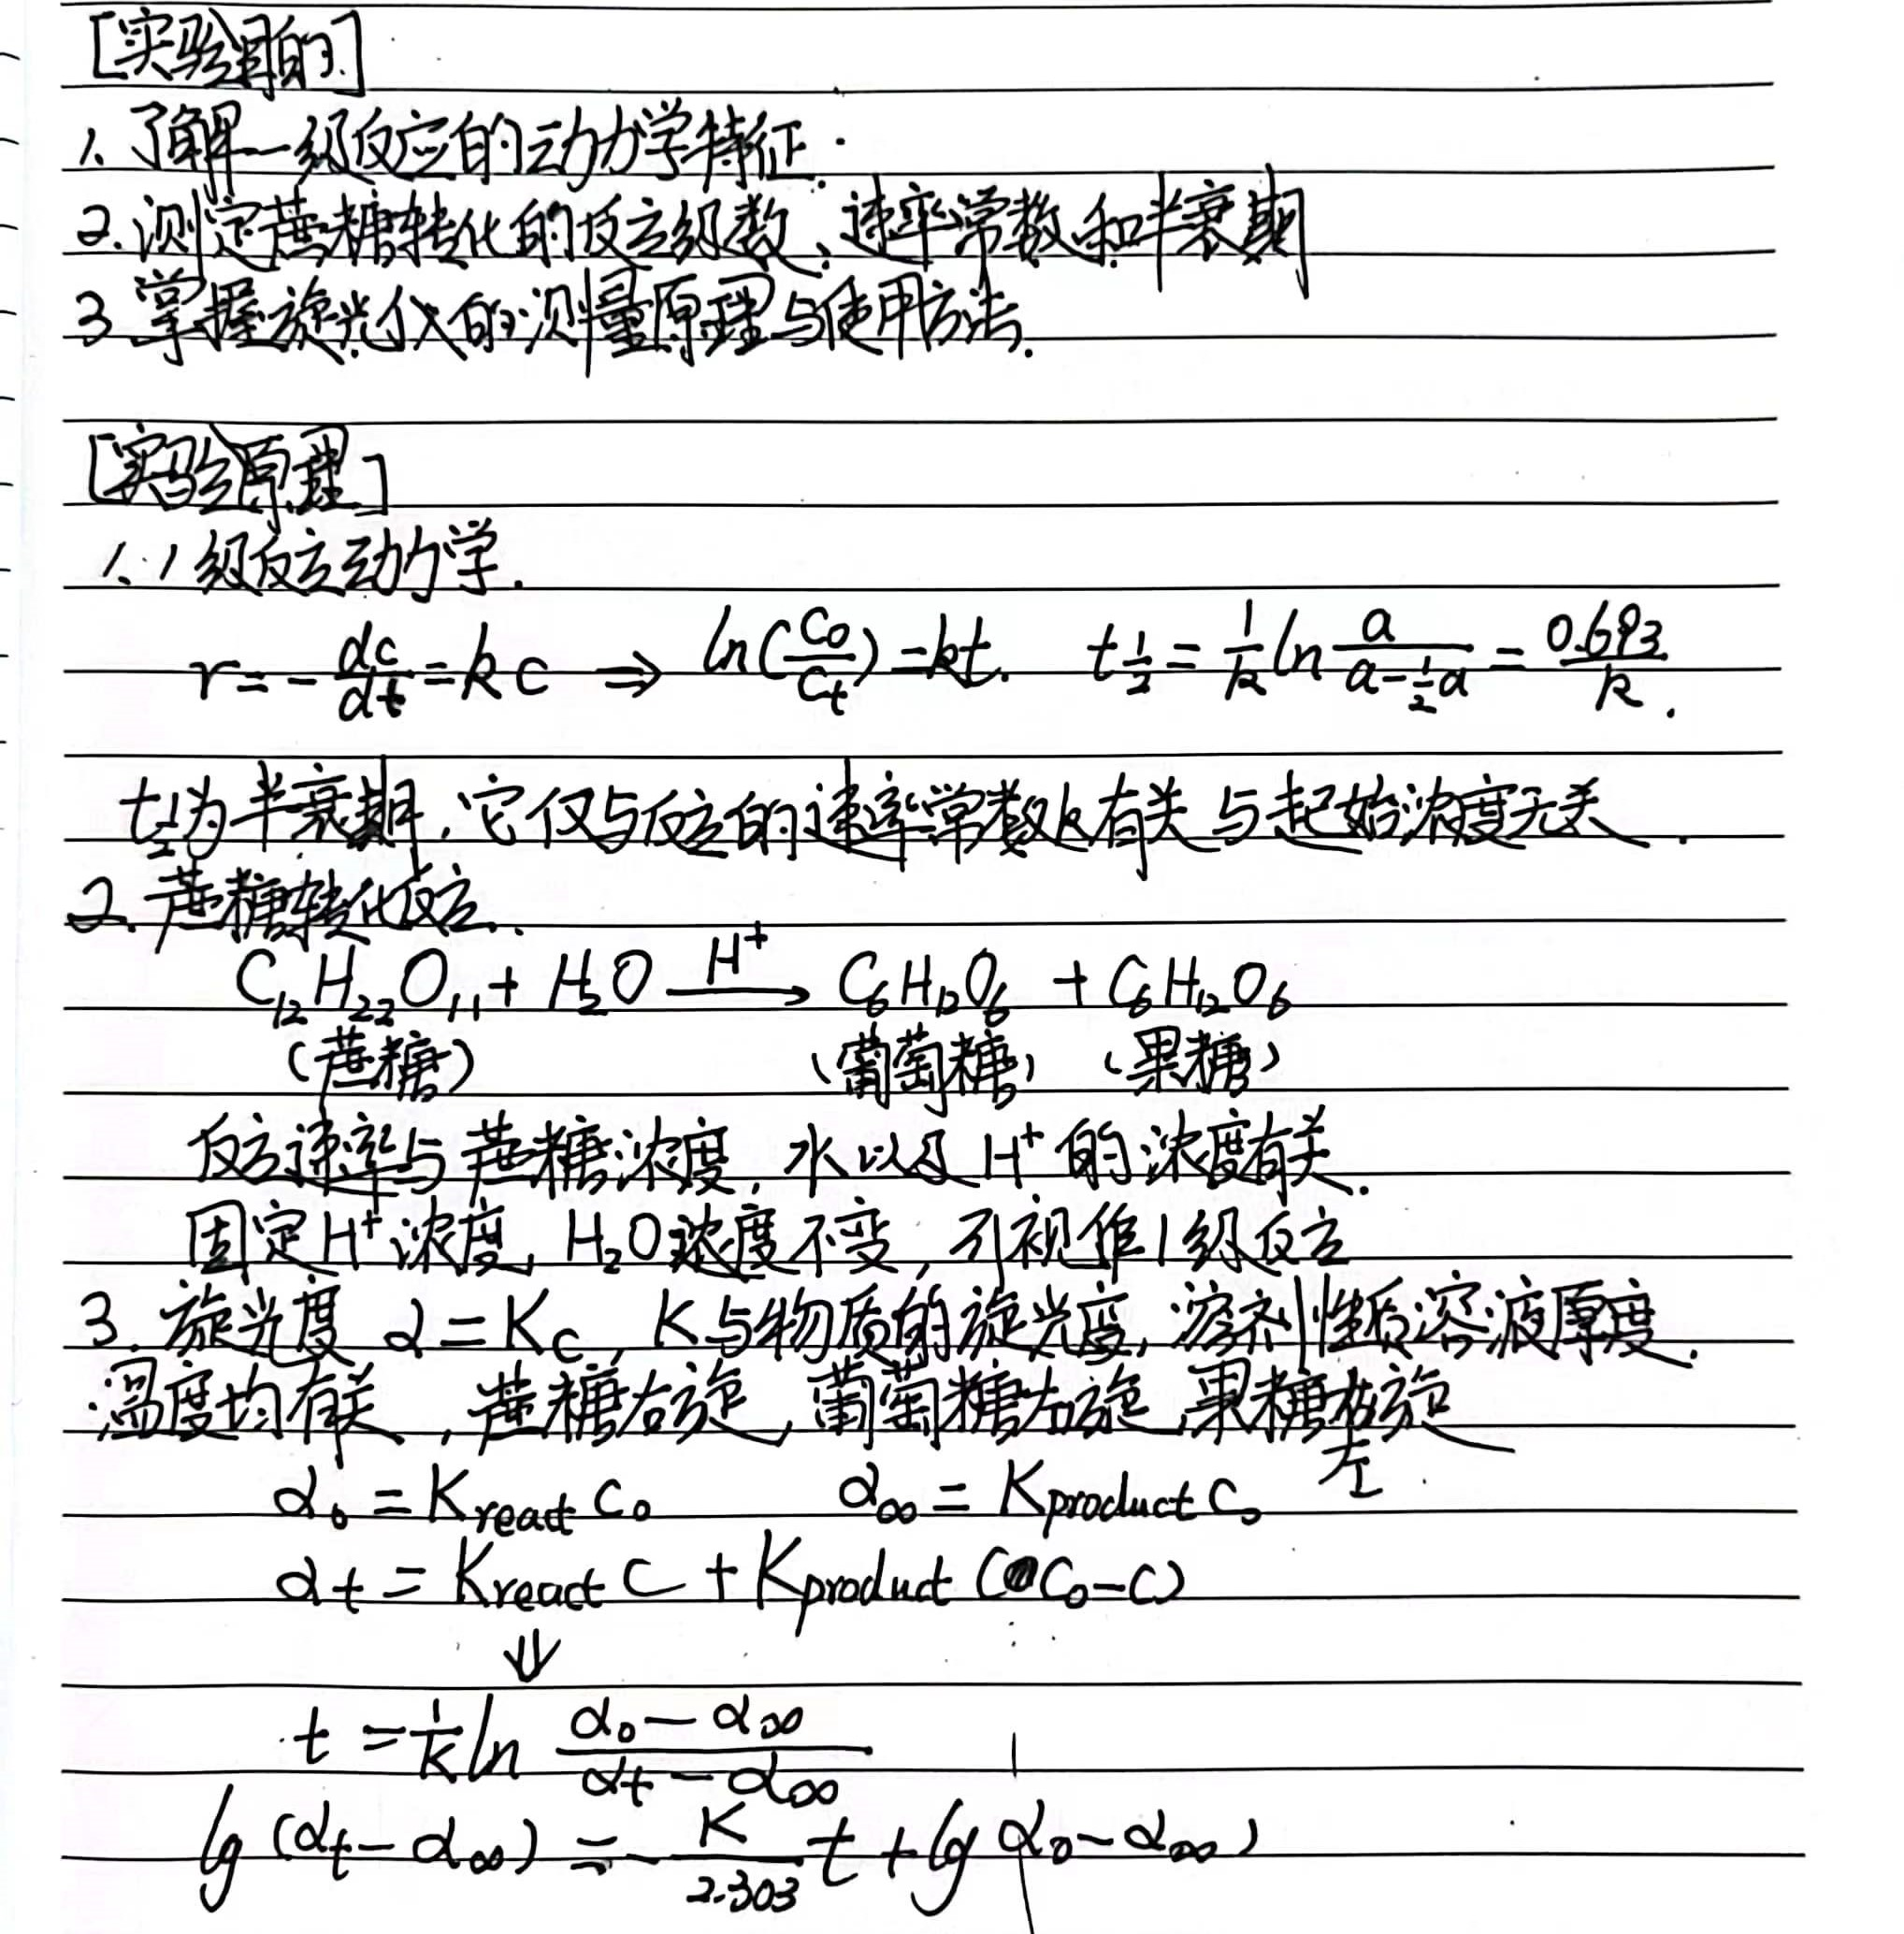
\includegraphics[width = .70\textwidth]{image/yxbg_1.jpg}
    \caption{实验的目的、原理}\label{1}
\end{figure}

\begin{figure}[htbp]
    \centering
    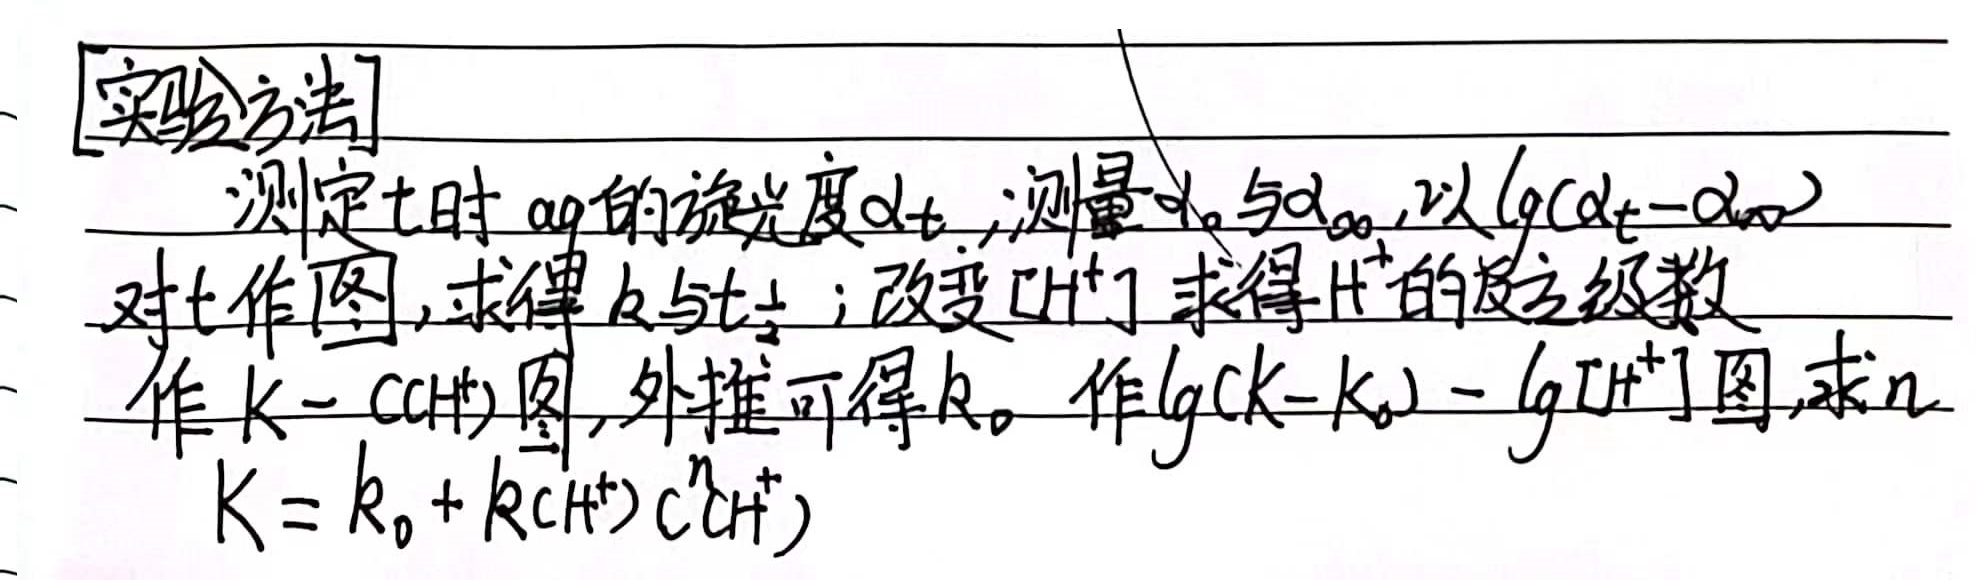
\includegraphics[width = .70\textwidth]{image/yxbg_2.jpg}
    \caption{实验的方法}\label{b}
\end{figure}

\section{实验部分}

\subsection{实验步骤}

实验步骤详见预习报告图~\ref{4} 。

\begin{figure}[htbp]
    \centering
    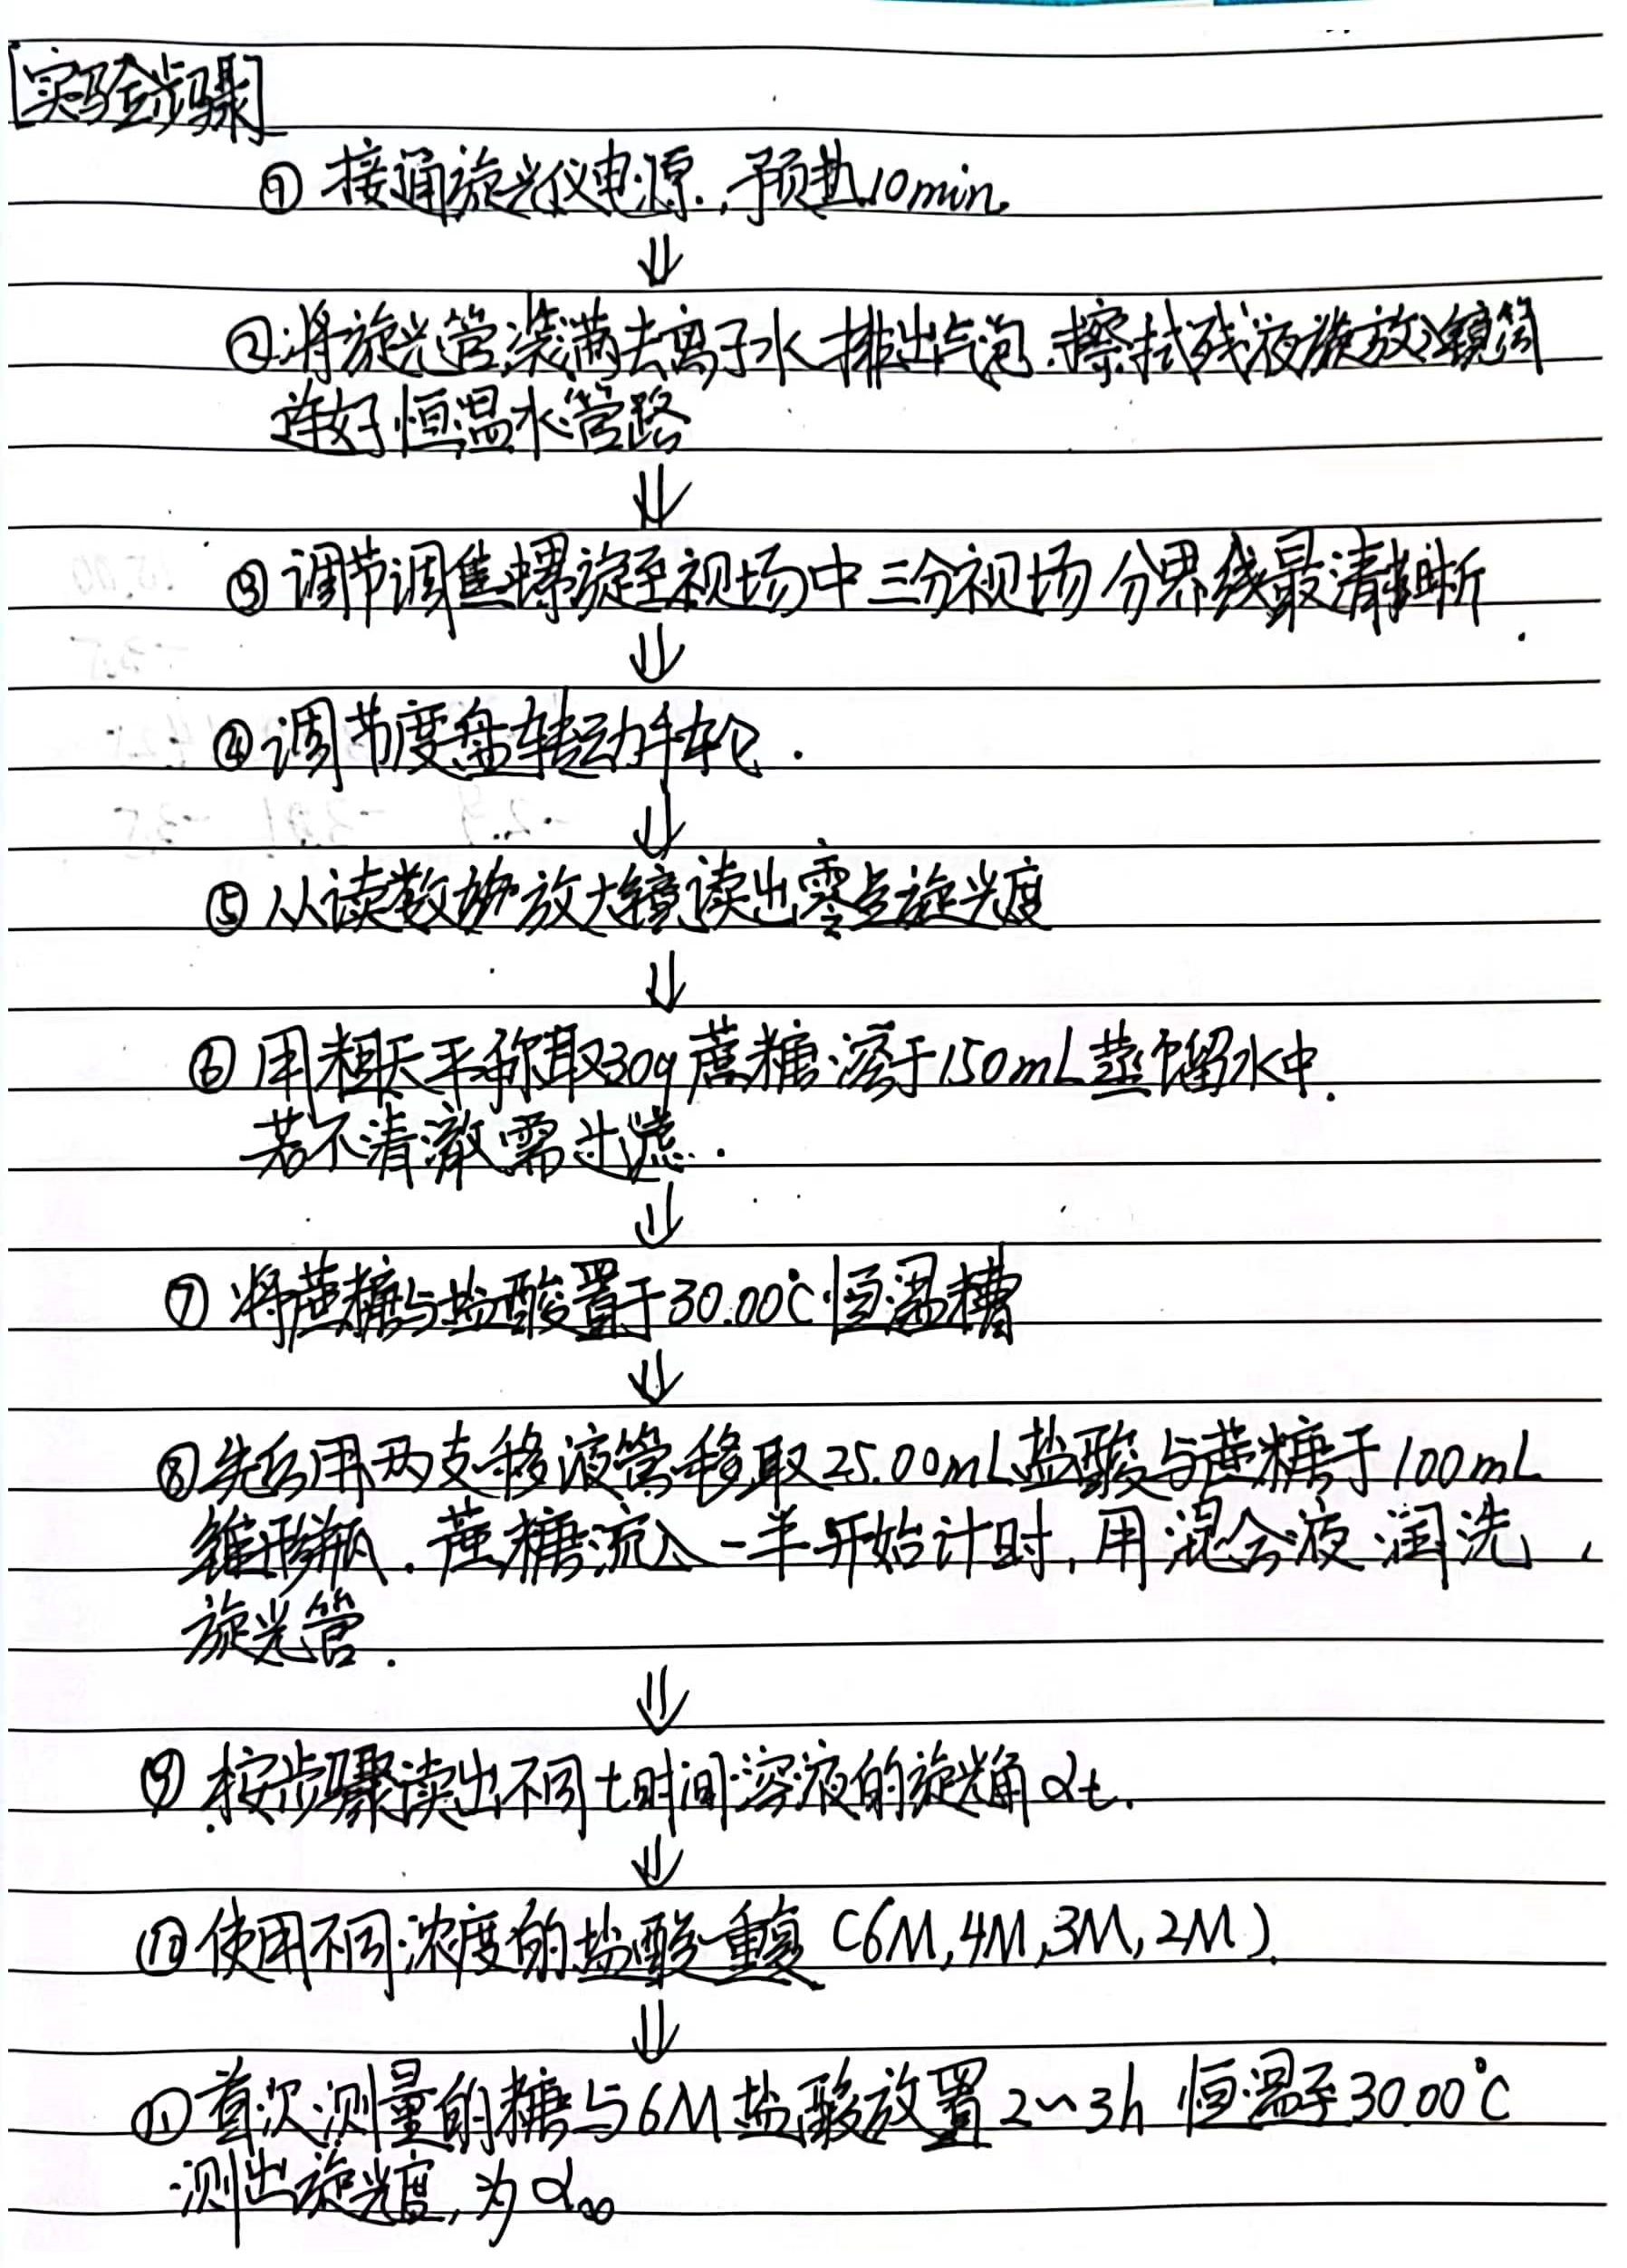
\includegraphics[width = .70\textwidth]{image/yxbg_3.jpg}
    \caption{实验步骤}\label{4}
\end{figure}

\subsection{仪器与药品}

\begin{enumerate} %有序列表
    \item 试剂 \\ 蔗糖(AR),盐酸(3.12 mol/L,4.19 mol/L,6.16 mol/L)。
    
    \item 仪器 \\ 旋光仪,秒表,恒温旋光管,500 mL 烧杯,25.00 mL 移液管,100 mL 磨口锥形瓶
    ,100 mL 量筒,水浴装置,0.01 g 电子台秤。
\end{enumerate}

\section{实验现象与数据处理}

\subsection{准备工作}

首先将恒温旋光管加满去离子水,测定旋光仪的零点。测定三次取得平均值为
$$ \alpha_0 = -0.1\degree $$

称量30.06 g蔗糖溶解于150 mL去离子水中得到蔗糖溶液。

\subsection{测定旋光度}
当盐酸浓度为 3.12 mol/L 时,测量旋光度随时间的变化如表 \ref{5}。

\begin{table}[h]
    \centering
    \caption{测定 M = 3.12 mol/L 的旋光度}
    \label{5}
    \begin{tabular}{cccc|cccc}
    \hline
    t/s & \multicolumn{1}{l}{$\rm \alpha_t / \degree$} & $\rm \alpha_t - \alpha_\infty / \degree$ & \multicolumn{1}{l|}{$\rm lg(\alpha_t-\alpha_\infty)$} & t/s & \multicolumn{1}{l}{$\rm \alpha_t / \degree$} & $\rm \alpha_t - \alpha_\infty / \degree$ & \multicolumn{1}{l}{$\rm lg(\alpha_t-\alpha_\infty)$} \\ \hline
    153 & 12.5 & 17.1 & 1.233 & 664 & 5.9 & 10.5 & 1.021 \\
    212 & 10.3 & 14.9 & 1.173 & 702 & 5.8 & 10.4 & 1.017 \\
    282 & 9.8  & 14.4 & 1.158 & 779 & 4.9 & 9.5  & 0.978 \\
    390 & 8.4  & 13.0 & 1.114 & 810 & 5.1 & 9.7  & 0.987 \\
    447 & 8.1  & 12.7 & 1.104 & 870 & 4.5 & 9.1  & 0.959 \\
    542 & 7.1  & 11.7 & 1.068 & 920 & 3.8 & 9.1  & 0.924 \\
    612 & 6.3  & 10.9 & 1.037 &     &     & &       \\ \hline
    \end{tabular}
\end{table}

当盐酸浓度为 4.19 mol/L 时,测量旋光度随时间的变化如表 \ref{6}。
\begin{table}[h]
    \centering
    \caption{测定 M = 4.19 mol/L 的旋光度}
    \label{6}
    \begin{tabular}{cccc|cccc}
    \hline
    t/s & \multicolumn{1}{l}{$\rm \alpha_t / \degree$} & $\rm \alpha_t - \alpha_\infty / \degree$ & \multicolumn{1}{l|}{$\rm lg(\alpha_t-\alpha_\infty)$} & t/s & \multicolumn{1}{l}{$\rm \alpha_t / \degree$} & $\rm \alpha_t - \alpha_\infty / \degree$ & \multicolumn{1}{l}{$\rm lg(\alpha_t-\alpha_\infty)$} \\ \hline
    139 & 9.5 & 14.1 & 1.149 & 510 & 4.5 & 9.1& 0.959 \\
    191 & 9.2 & 13.8 & 1.140 & 540 & 4.1 & 8.7& 0.940 \\
    249 & 8.9 & 13.5 & 1.130 & 579 & 3.5 & 8.1& 0.908 \\
    282 & 8.2 & 12.8 & 1.107 & 630 & 3.1 & 7.7& 0.886 \\
    302 & 7.8 & 12.4 & 1.093 & 680 & 2.4 & 7.0& 0.845 \\
    379 & 6.1 & 10.7 & 1.029 & 729 & 2.0 & 6.6& 0.820 \\
    418 & 5.5 & 10.1 & 1.004 & 786 & 1.7 & 6.3& 0.799 \\
    453 & 5.2 & 9.8  & 0.991 & 855 & 1.2 & 5.8& 0.763 \\
    486 & 5.0 & 9.6  & 0.982 & 900 & 0.7 & 5.3& 0.724 \\ \hline
    \end{tabular}
\end{table}

当盐酸浓度为 6.16 mol/L 时,测量旋光度随时间的变化如表 \ref{7}。
\begin{table}[h]
    \centering
    \caption{测定 M = 6.16 mol/L 的旋光度}
    \label{7}
    \begin{tabular}{cccc|cccc}
    \hline
    t/s & \multicolumn{1}{l}{$\rm \alpha_t / \degree$} & $\rm \alpha_t - \alpha_\infty / \degree$ & \multicolumn{1}{l|}{$\rm lg(\alpha_t-\alpha_\infty)$} & t/s & \multicolumn{1}{l}{$\rm \alpha_t / \degree$} & $\rm \alpha_t - \alpha_\infty / \degree$ & \multicolumn{1}{l}{$\rm lg(\alpha_t-\alpha_\infty)$} \\ \hline
    160 & 6.6  &11.2 & 1.049 & 514 & -1.1 & 3.5& 0.544 \\
    198 & 5.5  &10.1 & 1.004 & 543 & -1.4 & 3.2& 0.505 \\
    220 & 4.2  &8.8  & 0.944 & 588 & -1.8 & 2.8& 0.447 \\
    266 & 3.5  &8.1  & 0.908 & 632 & -2.2 & 2.4& 0.380 \\
    313 & 3.0  &7.6  & 0.881 & 675 & -2.7 & 1.9& 0.279 \\
    350 & 2.0  & 6.6 & 0.820 & 744 & -3.0 & 1.6& 0.204 \\
    390 & 0.7  &5.3  & 0.724 & 774 & -3.2 & 1.4& 0.146 \\
    420 & 0.5  &5.1  & 0.708 & 816 & -3.3 & 1.3& 0.114 \\
    453 & -0.1 & 4.5 & 0.653 & 868 & -3.5 & 1.1& 0.041 \\
    490 & -0.8 &3.8  & 0.580 & 900 & -3.6 & 1.0& 0.000 \\ \hline
    \end{tabular}
\end{table}

将蔗糖溶液与6.16 mol/L盐酸混合3小时以上后测定其旋光度即为$\rm \alpha_\infty$。测定三次取平均值为
$$\alpha_\infty = -4.7\degree$$

\subsection{旋光度数据处理}
将 $\rm \alpha_t$ 对 $t$ 作图如图 \ref{7.5} 所示。可以发现, $\rm \alpha_t$ 对 $t$ 无显著线性关系,随着时间的推移旋光度的变化均越来越慢。

\begin{figure}[htbp]
    \centering
    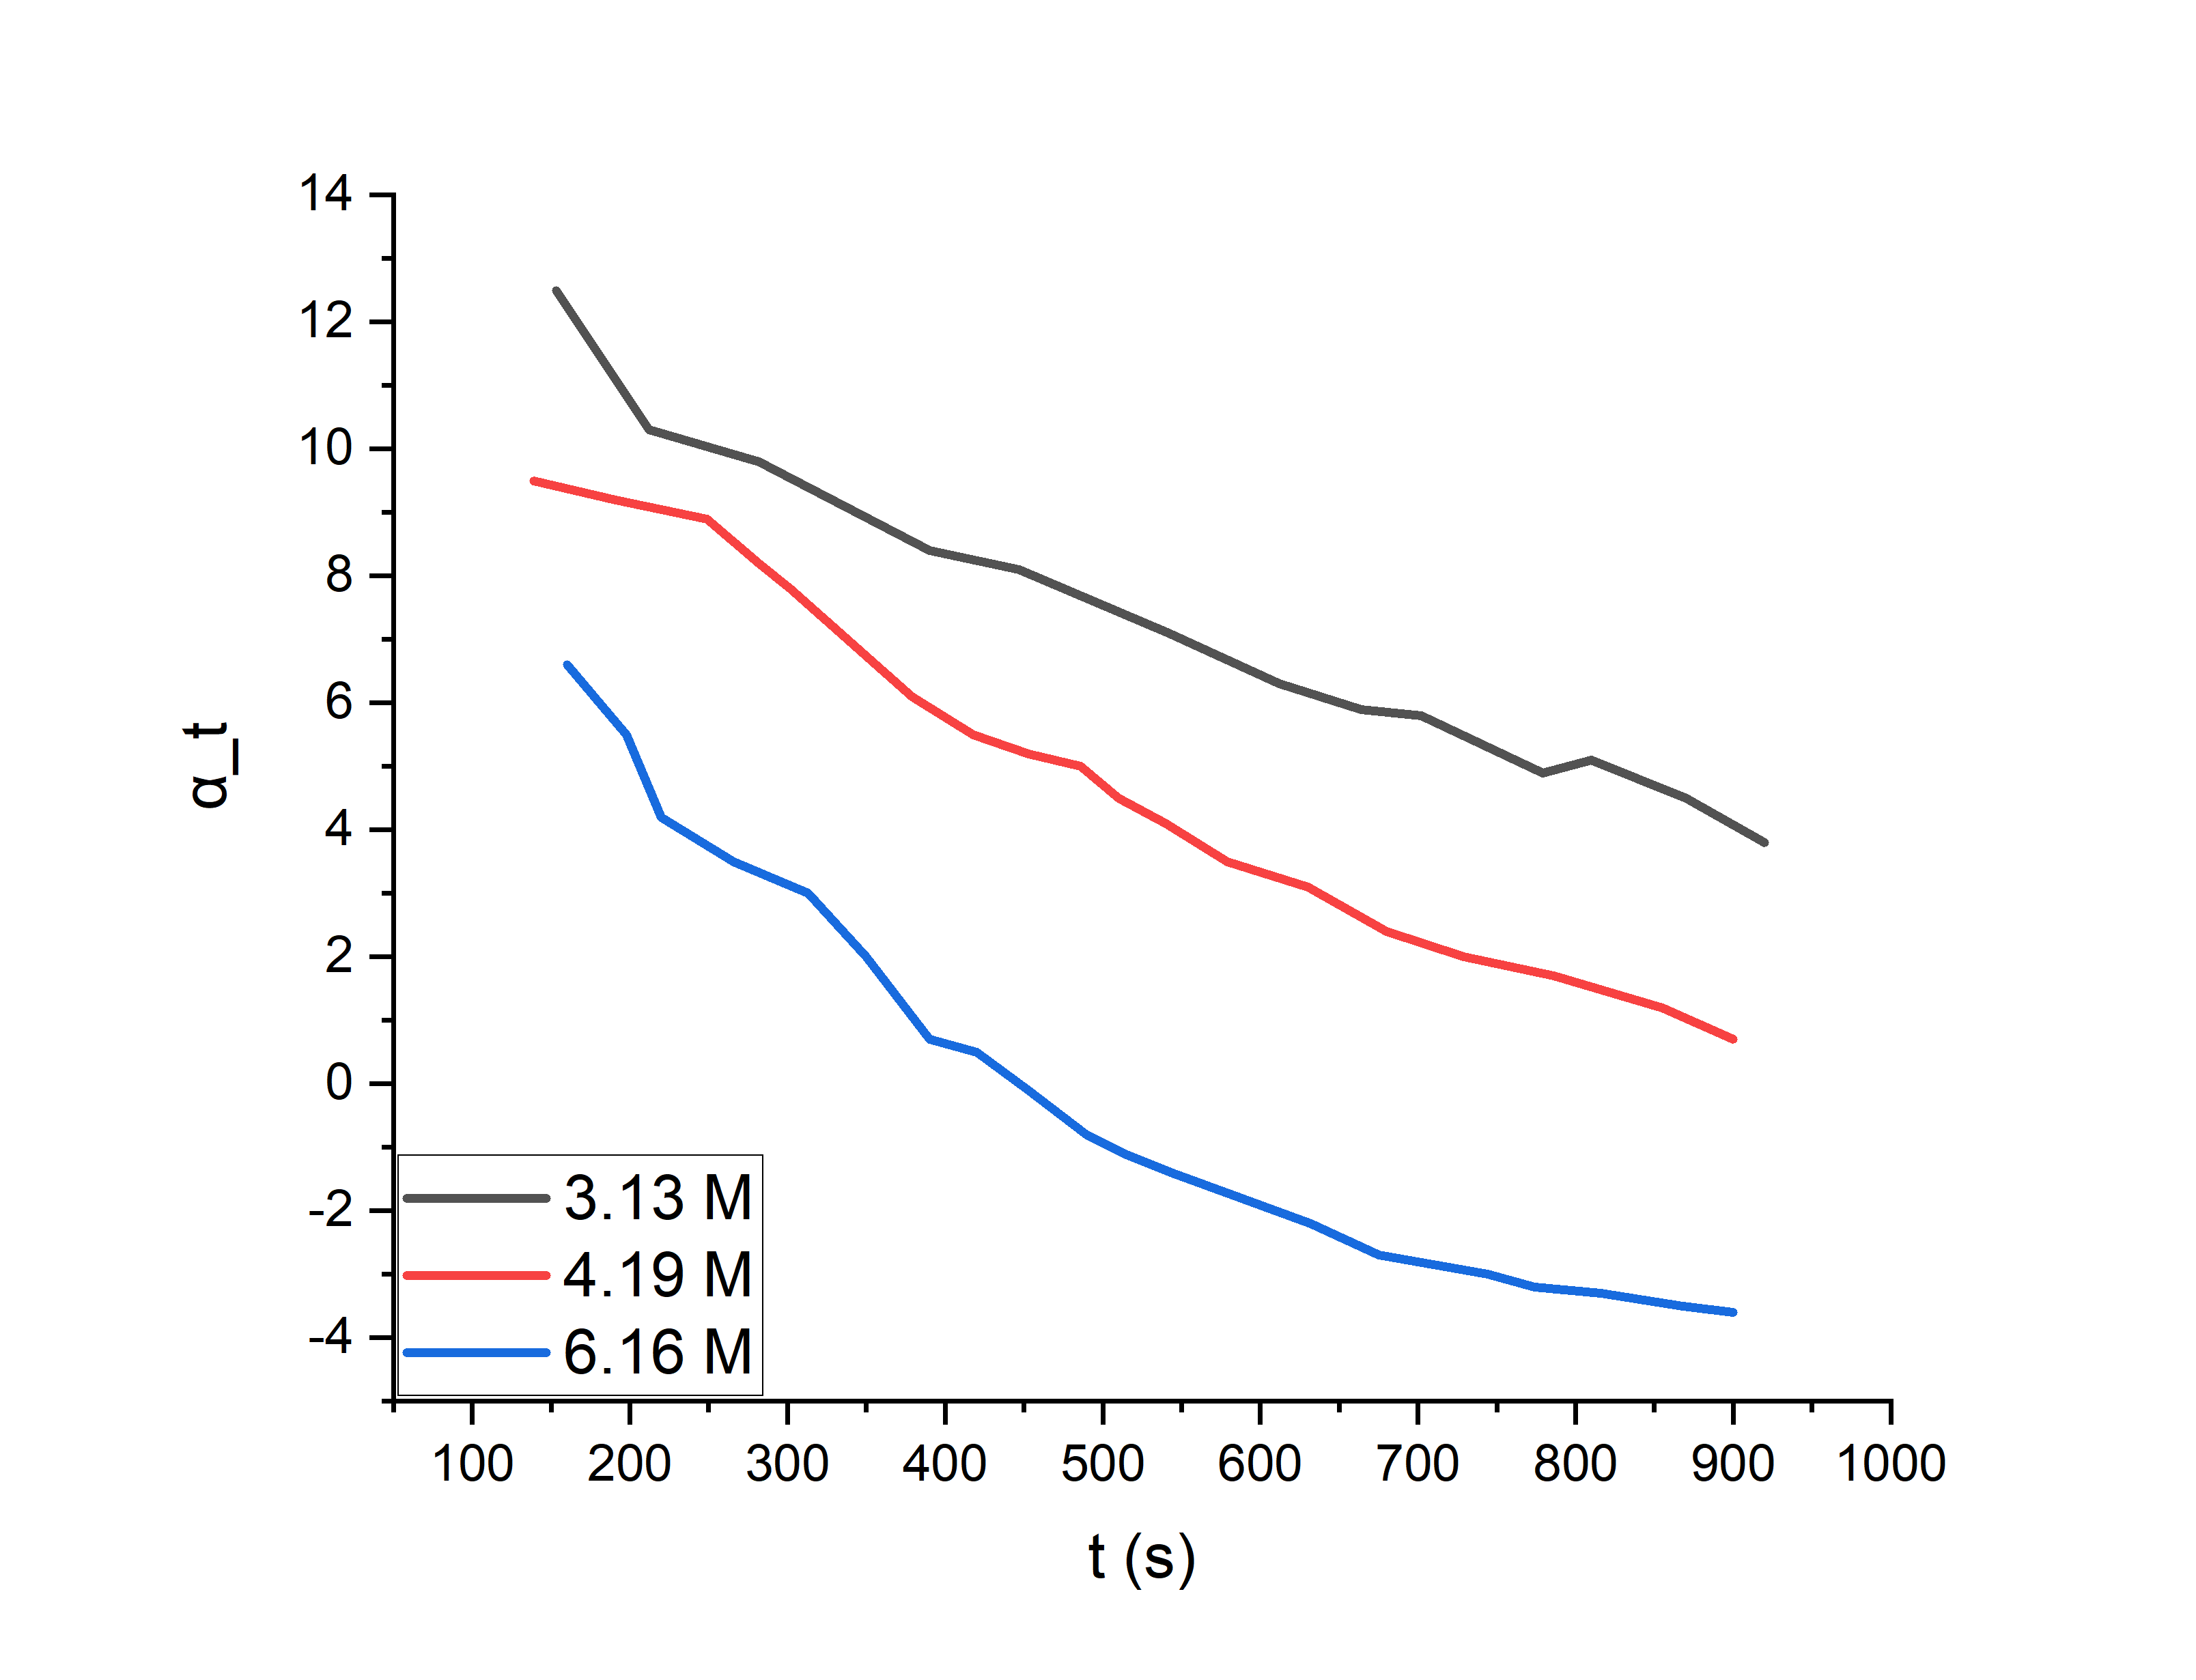
\includegraphics[width = .70\textwidth]{image/Graph9.png}
    \caption{三种氢离子浓度下的$\alpha_t - t $图}\label{7.5}
\end{figure}


将 $\rm \lg(\alpha_t - \alpha_\infty)$ 对 $t$ 作图,并进行线性回归如图 \ref{8} 所示,线
性回归的结果如下所示。

$\rm [H^+] = 3.12\ M$时,
$$
\lg(\alpha_t - \alpha_\infty) = (1.264 \pm  0.008) + (-3.602 \pm  0.127) \cdot  10^{-4} \cdot  t \quad R^2=0.985	
$$

$\rm [H^+] = 4.16\ M$时,
$$
\lg(\alpha_t - \alpha_\infty) = (1.258 \pm  0.007) + (-5.892 \pm  0.124) \cdot  10^{-4} \cdot  t \quad R^2=0.993
$$

$\rm [H^+] = 6.16\ M$时,
$$
\lg(\alpha_t - \alpha_\infty) = (1.299 \pm  0.011) + (-14.60 \pm  0.196) \cdot  10^{-4} \cdot  t \quad R^2=0.997	
$$

在不同氢离子浓度下,$\rm \lg(\alpha_t - \alpha_\infty)$ 对 $t$ 的线性关系较好,可以判断该反应对蔗糖浓度为一级反应。
\begin{figure}[htbp]
    \centering
    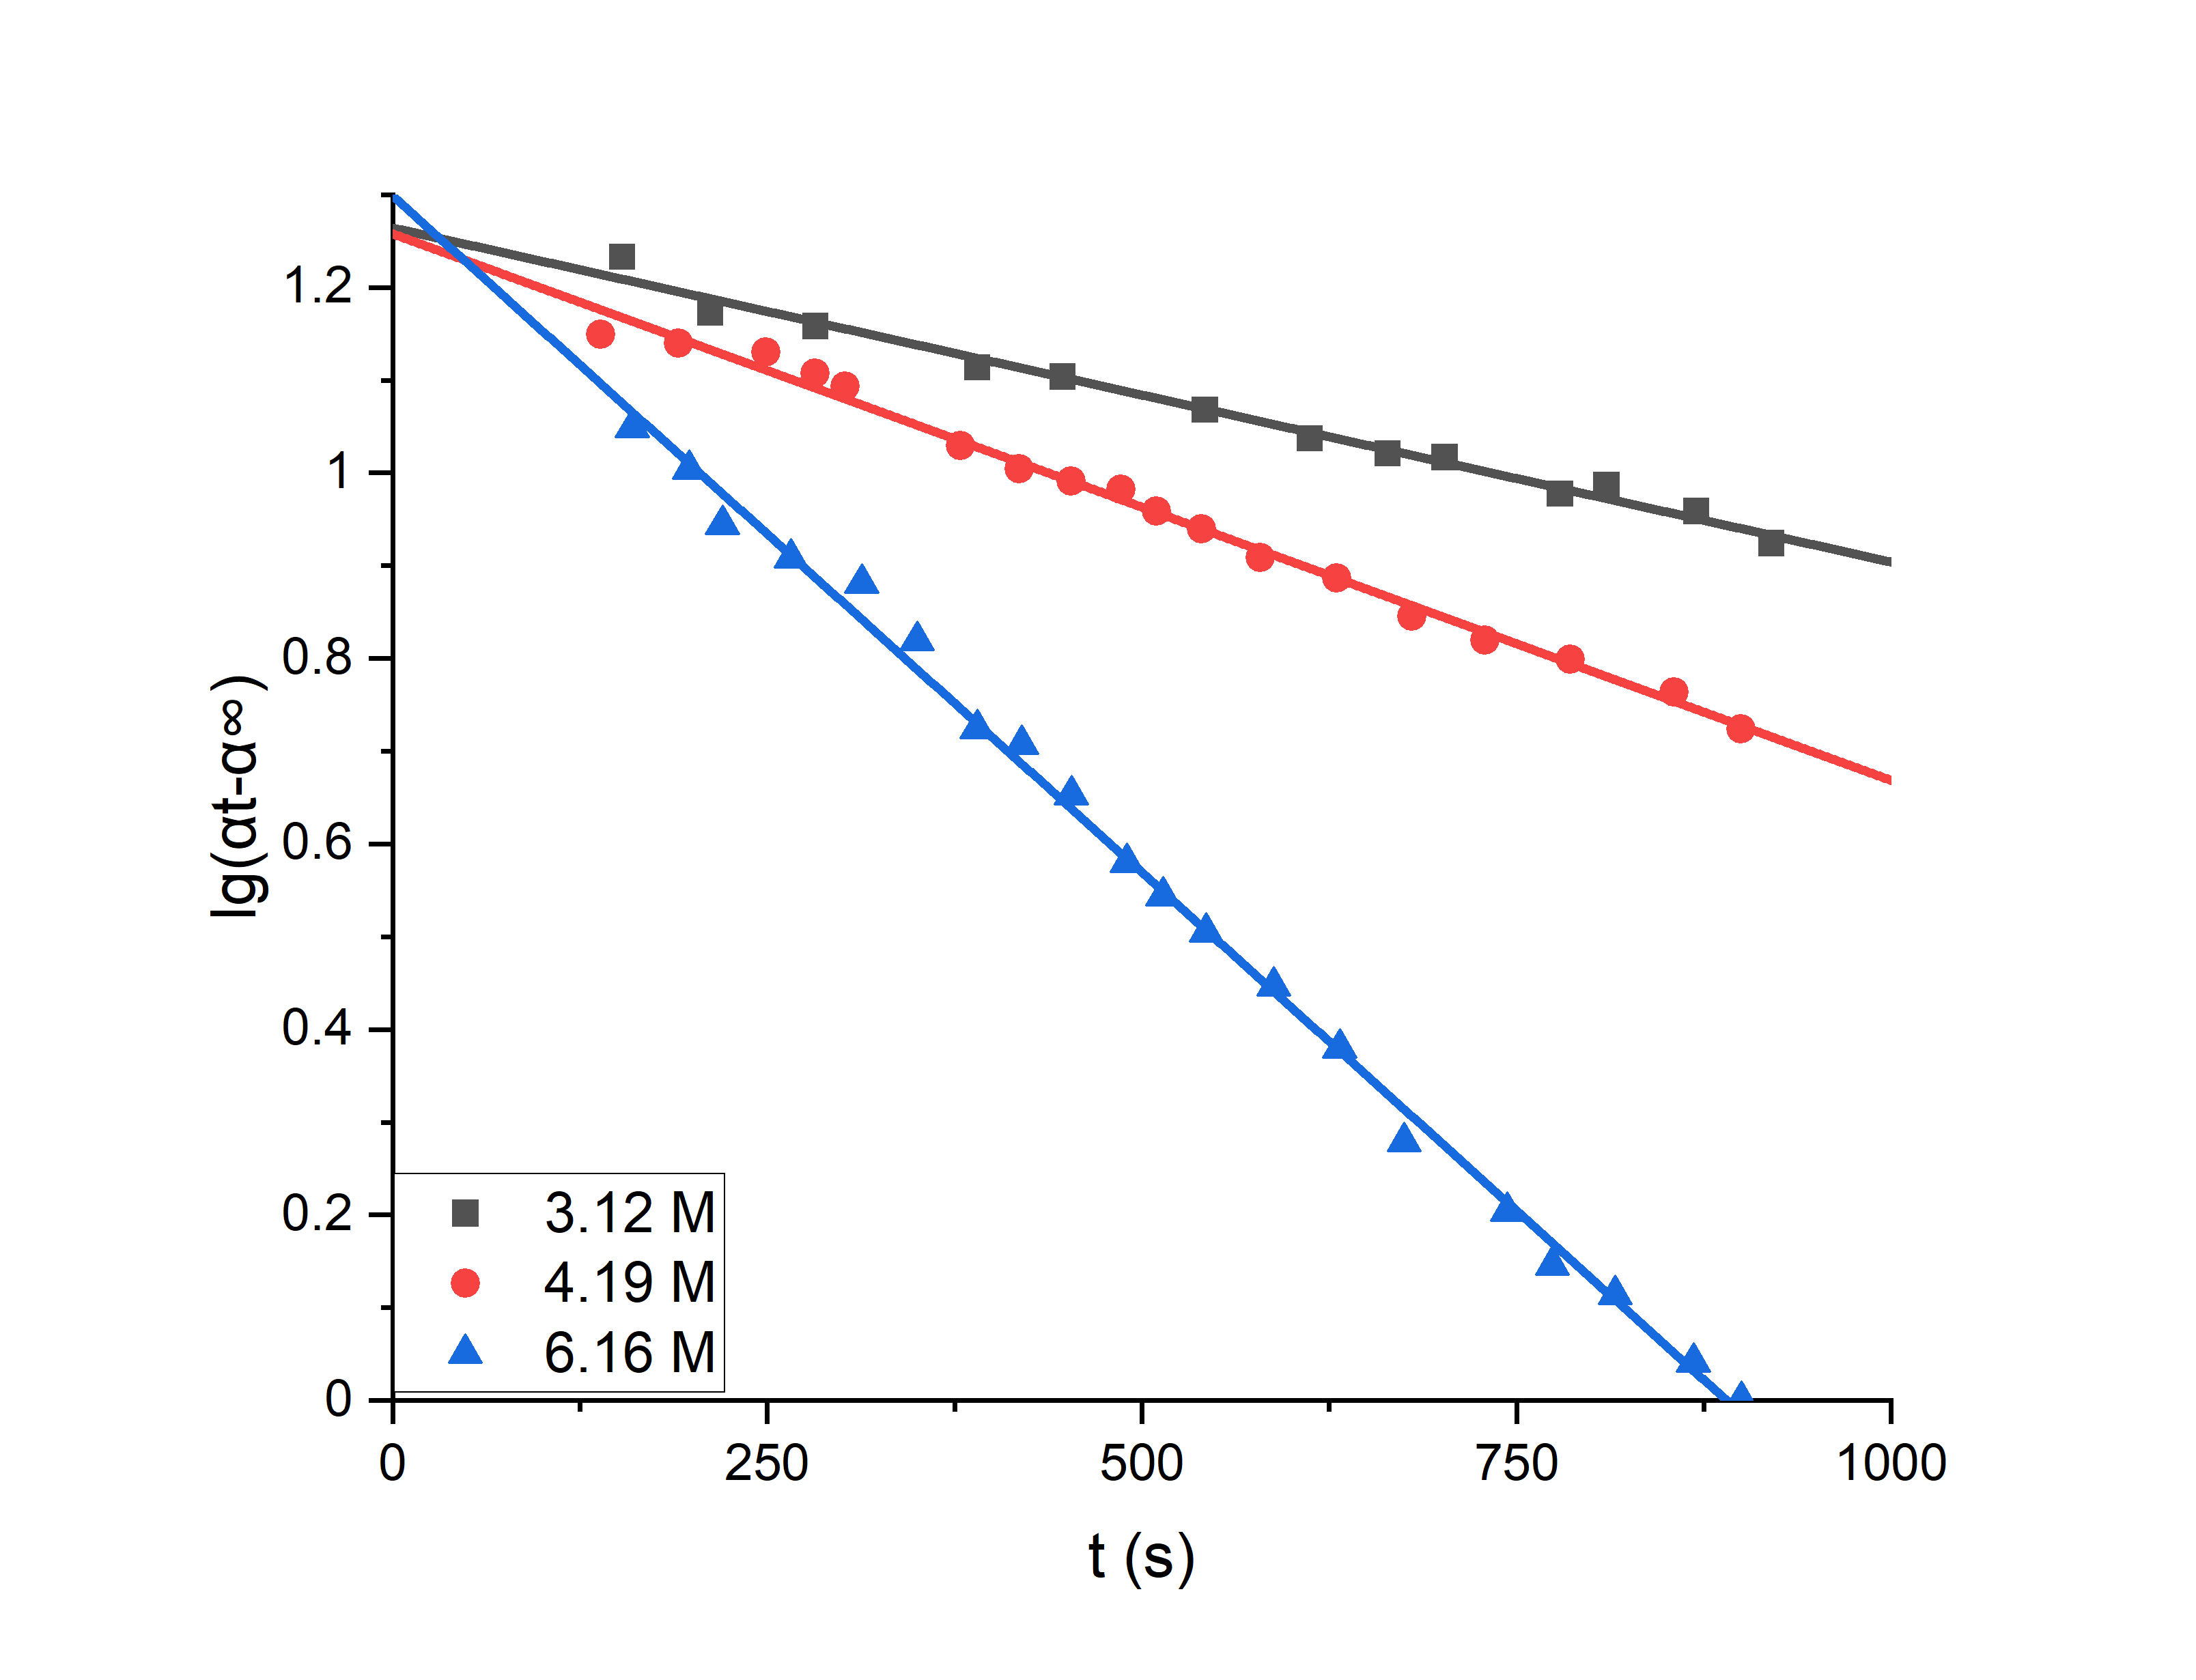
\includegraphics[width = .70\textwidth]{image/Graph6.png}
    \caption{ 三种氢离子浓度下的$lg(\alpha_t - \alpha_\infty) - t $图}\label{8}
\end{figure}

由数学推导可知
$$
lg(\alpha_t - \alpha_\infty) = -\frac{k}{2.303}t + lg(\alpha_0 - \alpha_\infty)
$$
$$
t_{1/2} = \frac{ln2}{k}
$$
因此可以计算得到三种氢离子浓度下的反应速率常数与半衰期如下表 \ref{10} 。

\begin{table}[h]
    \centering
    \caption{三种氢离子浓度下的反应的速率常数与半衰期}
    \label{10}
    \begin{tabular}{ccc}\hline
    $[H^+]/M$& 速率常数$ / s^{-1}$ & 半衰期$/s$ \\ \hline
    3.12                         & 8.295$\ \cdot\ 10^{-4}$                  & 835.40 \\
    4.19                         & 1.357$\ \cdot\ 10^{-3}$               & 510.71 \\
    6.16                         & 3.362$\ \cdot\ 10^{-3}$                & 206.10 \\\hline
    \end{tabular}
\end{table}

如考虑氢离子对反应速率的影响,则有
$$
k = k_0 + k({\rm H^+}) \cdot {\rm [H^+]}^n
$$


由于碱性条件下蔗糖溶液稳定,不会分解,因此近似认为 $k_0=0$,因此
$$
\ln(k-k_0)=\ln(k({\rm H^+})) + n \cdot \ln({\rm [H^+]})
$$

其中 $k_0$ 为 $\rm [H^+]$ 趋于 0 时的速率常数,$ k({\rm H^+})$ 为酸催化速率常数,k 为表观速率常数,n 为氢离子的反应级数
。由表 \ref{10} 作 $\ln(k-k_0)$ 对 $\ln({\rm [H^+]})$ 的图,并进行线性回归如图 \ref{11} 所示,拟合直线为
$$
ln(k-k_0) = -9.496 \pm 0.2879 + (2.072 \pm 0.193 ) \ln({\rm [H^+]}) \quad R^2 = 0.99137
$$

\begin{figure}[h]
    \centering
    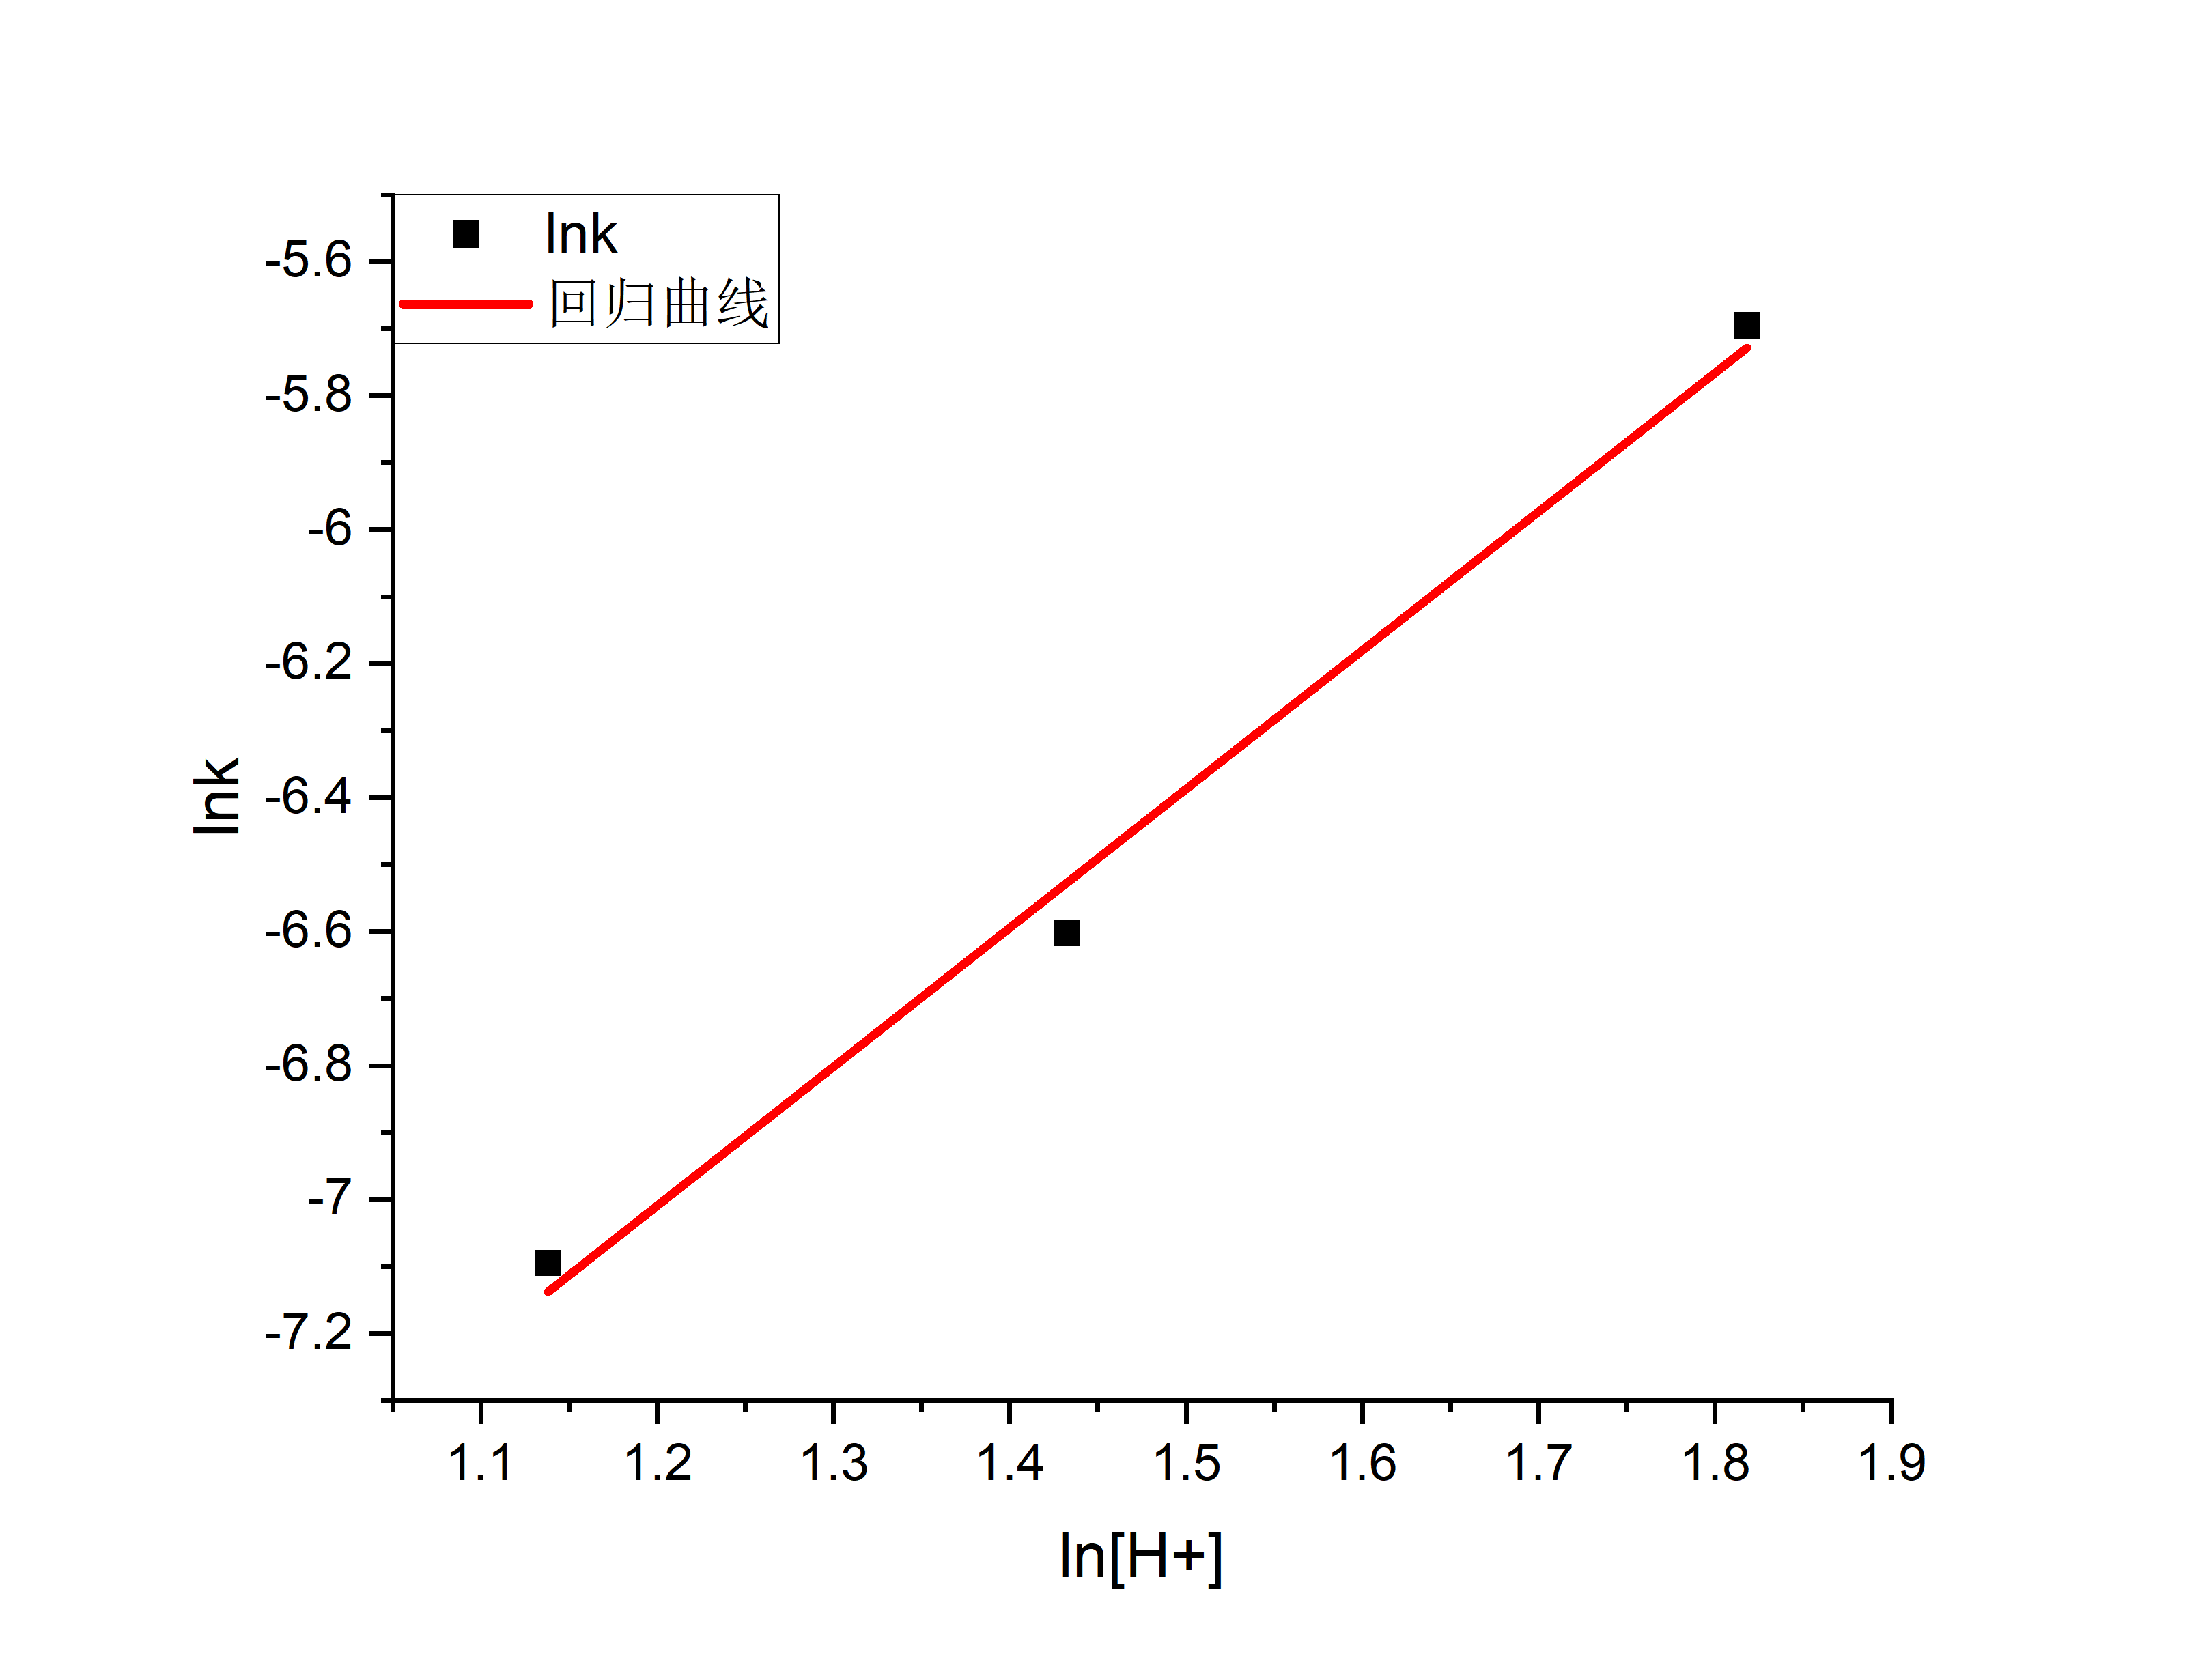
\includegraphics[width = .60\textwidth]{image/Graph13.png}
    \caption{ 三种氢离子浓度下的$\ln(k-k_0) - \ln({\rm [H^+]})$图}\label{11}
\end{figure}

线性回归曲线的斜率即为反应级数,$n = 2.072 \approx  2$,因此氢离子的反应级数为 2。


\section{实验结果与讨论}

\subsection{讨论}

\subsubsection{另一种数据处理方式}

这里阐述一种不利用$\alpha_\infty$的数据处理方法。由于$c = c_0e^{-kt}$,可得
$$
c_1 - c_2 = c_0e^{-kt}(1-e^{-k \Delta t})
$$

对上式取对数,然后使用旋光角代替浓度 c 可得
$$
\lg(\alpha_1 - \alpha_2) = - \frac{k}{2.303}t + \lg[K_{反}c_0(1-e^{-k \Delta t})]
$$

我们取$\Delta t=370s$,以氢离子浓度为6.16 M为例,得到数据如下表所示

\begin{table}[h]
    \centering
    \caption{ M = 6.16 mol/L 的旋光度与差值对数值}
    \label{19}
    \begin{tabular}{ccccc}
    \hline
    t/s & $\alpha_1$ & $t+\Delta t/s$ & $\alpha_2$ & $\lg(\alpha_1-\alpha_2)$ \\ \hline
    160 & 6.6        & 530            & -1.4       & 0.90309                  \\
    198 & 5.5        & 568            & -1.8       & 0.863323                 \\
    220 & 4.2        & 590            & -1.8       & 0.778151                 \\
    266 & 3.5        & 636            & -2.2       & 0.755875                 \\
    313 & 3          & 683            & -2.7       & 0.755875                 \\
    350 & 2          & 720            & -2.9       & 0.690196                 \\
    390 & 0.7        & 760            & -3.2       & 0.591065                 \\
    420 & 0.5        & 790            & -3.2       & 0.568202                 \\
    453 & -0.1       & 823            & -3.3       & 0.50515                  \\
    490 & -0.8       & 860            & -3.5       & 0.431364                 \\
    514 & -1.1       & 884            & -3.6       & 0.39794                  \\ \hline
    \end{tabular}
\end{table}

作$\lg(\alpha_1-\alpha_2) - t$图如图 \ref{14}。得到回归直线为
$$
\lg(\alpha_1-\alpha_2) = 1.133 \pm 0.0298 + (-0.00138 \pm 8.218\cdot10^{-5}) t \quad R^2=0.9658
$$

\begin{figure}[h]
    \centering
    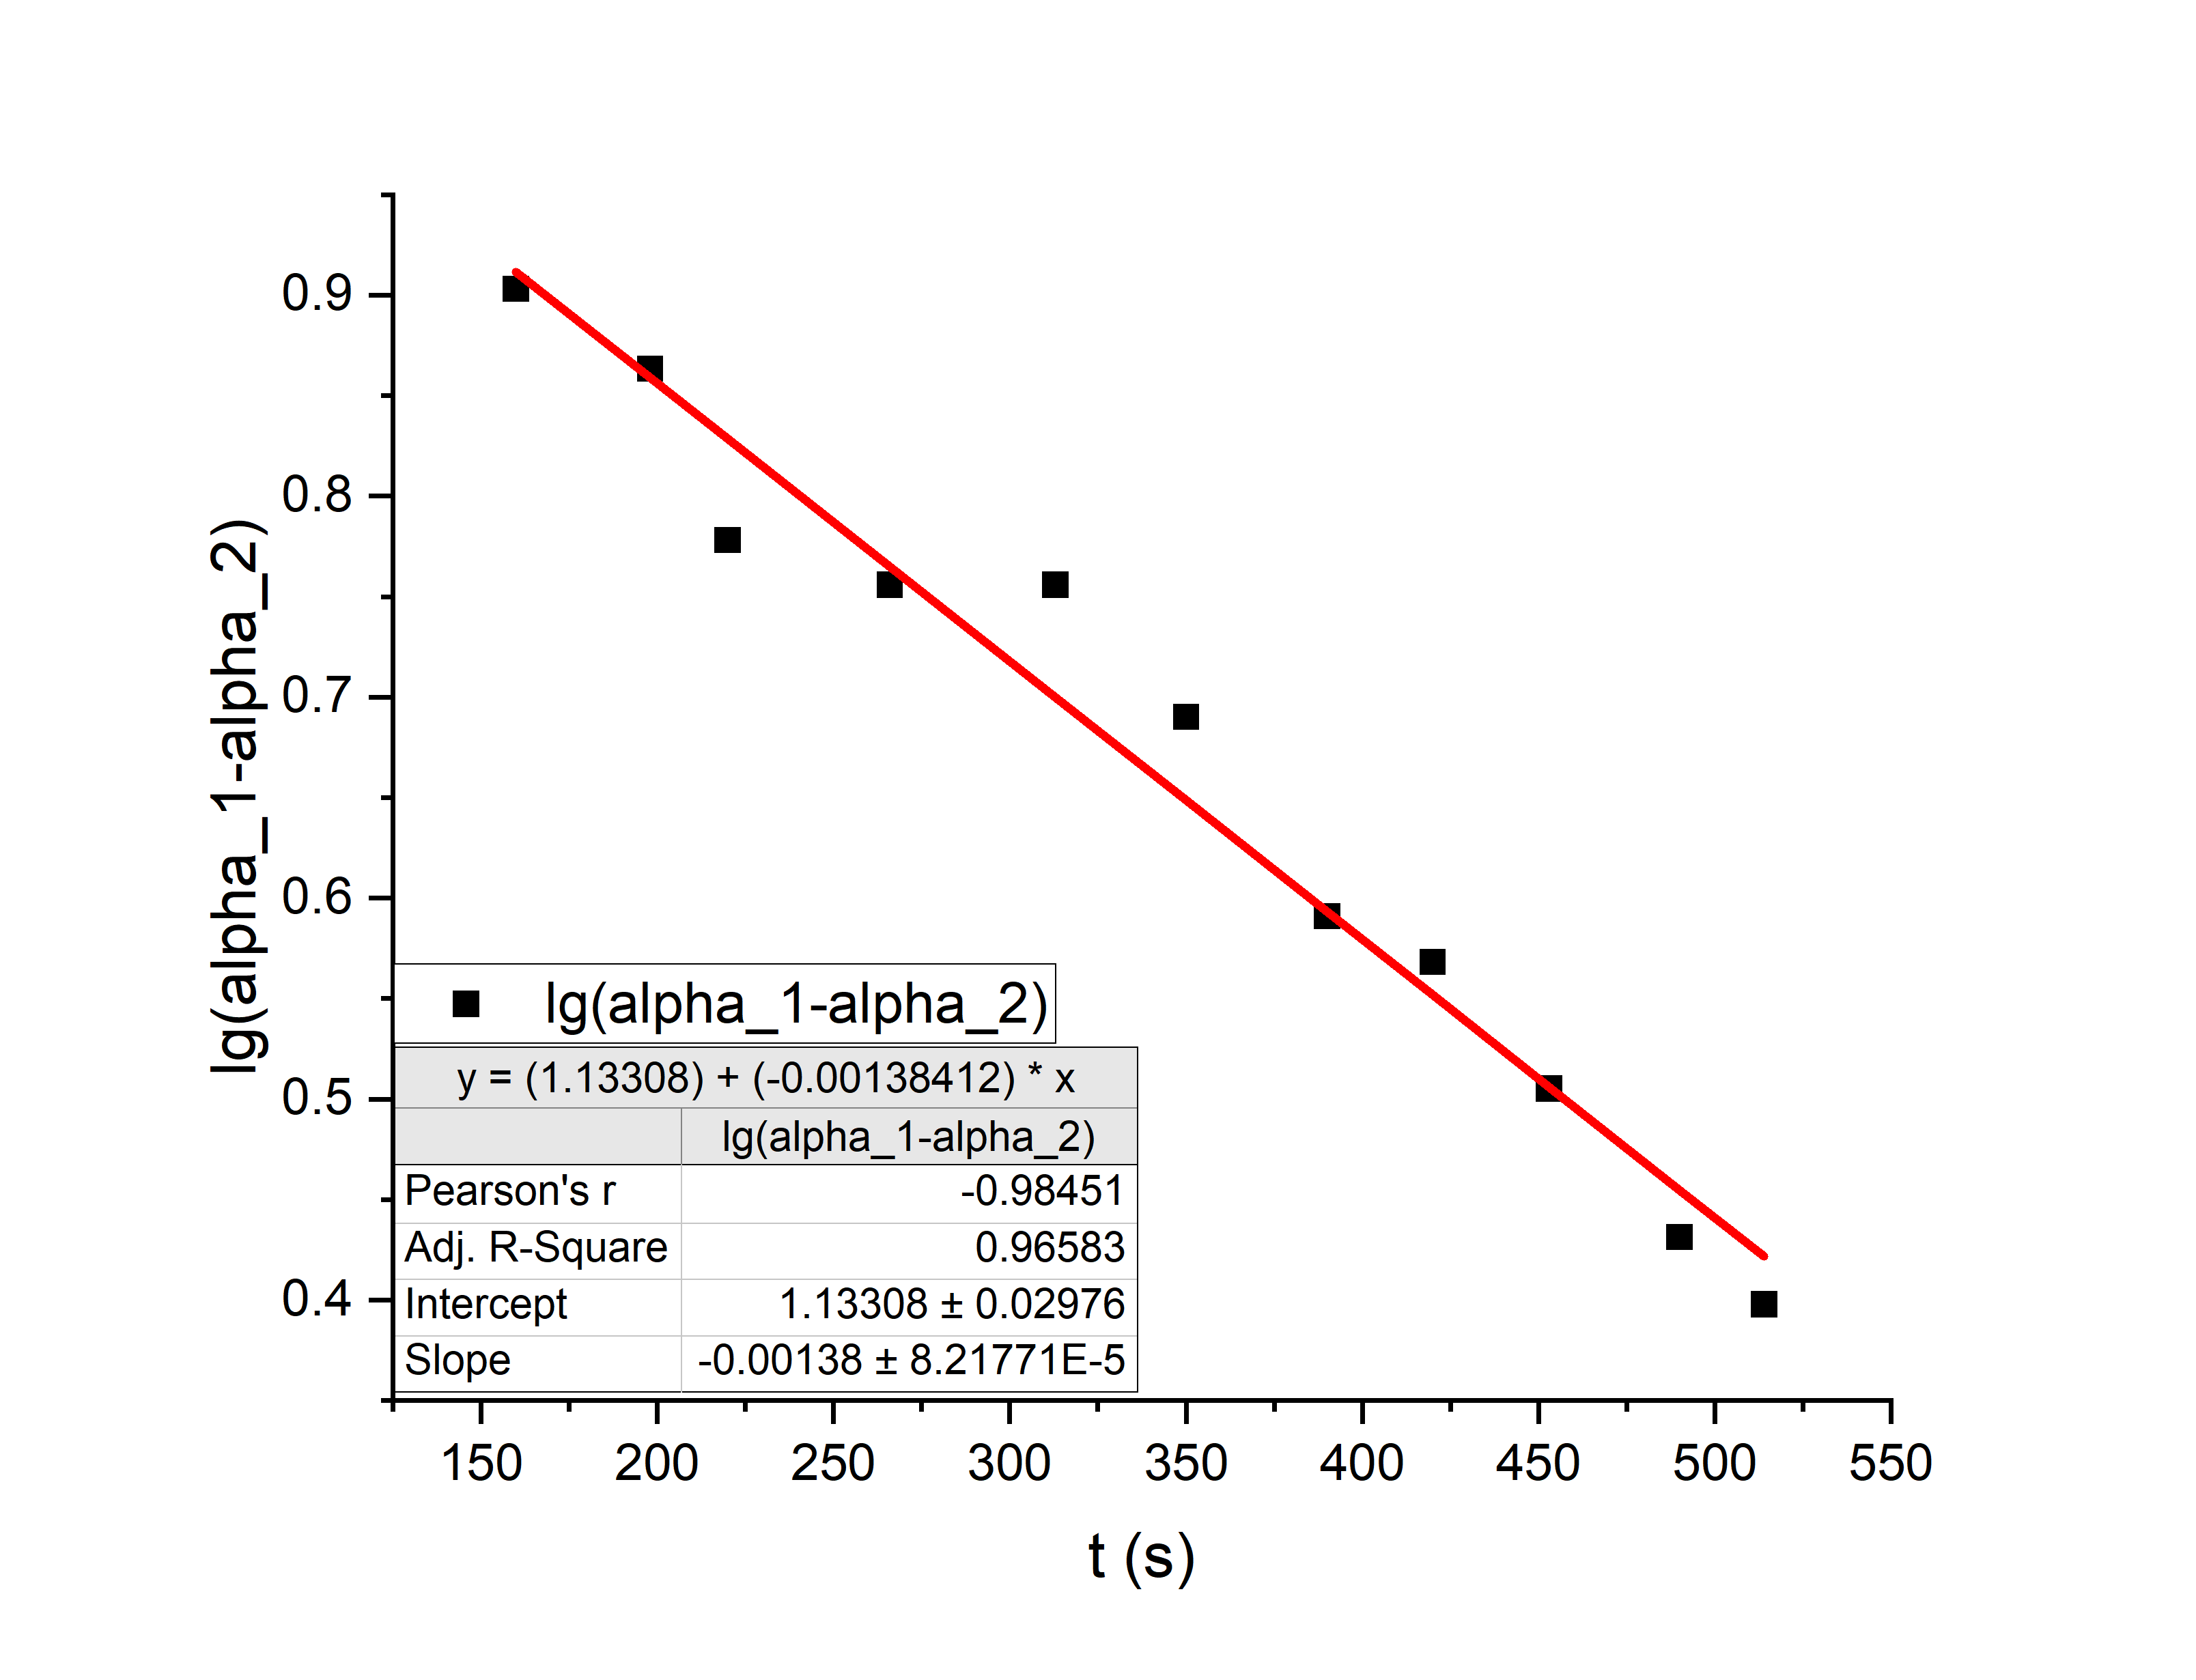
\includegraphics[width = .70\textwidth]{image/Graph15.png}
    \caption{$\rm [H^+]=6.16M$ 下 $\lg(\alpha_1-\alpha_2) - t$图}\label{14}
\end{figure}

由于测量时间的随机性,部分数据并不准确,取对应时间的临近值。因此得到的线性关系较为一般,但是也具有一定线性。由此可以得到 $k = 3.18\cdot10^{-5}$。与表4中的结果对比较为接近
,可以认为这是一种有效的反应速率常数的计算方法。

\subsubsection{误差的定性分析}

本实验操作简单,但是在旋光仪三分界限消失时,对应的螺旋测微器上是一段区域,而非一点。因此在这里存在误差。
同时,在测量时间上并不能完全看到视界消失时就记录对应的时间,因此时间记录上也存在误差。因此本次实验的线性程度并不很好,$R^2$在 0.985 - 0.997 之间。
这些误差可以通过提高操作熟练度,增加数据记录数量来提高准确度,三次测量的$R^2$逐次增加也可以佐证这一结论。

\subsection{结论}

本实验通过旋光度来确定溶液中蔗糖的浓度,将不易观测的物理量转化为可以测量的物理量。
并通过这种方法,较为精确地计算出蔗糖的反应级数,表观反应速率常数和半衰期以及氢离子的反应级数。
在报告中还阐述一种不利用$\alpha_\infty$的数据处理方法,也可以通过这种方法来得到蔗糖的表观反应速率常数。
通过误差分析,在操作熟练的基础上,旋光仪法是一种优良的测定反应动力学性质的方法。



\nocite{*}
\bibliography{reference}


\end{document}


%
%\section{实验目的}
%
%\begin{enumerate} %有序列表
%    \item 了解量子力学一维势阱模型
%    \item 了解紫外可见光谱仪的原理和构成
%    \item  学习紫外可见光谱仪的搭建和调试
%    \item 测定一些共轭分子的紫外可见光谱
%    \item 验证量子力学一维势阱公式
%\end{enumerate}
%
%\section{实验原理}
%
%\subsection{一维势阱中的能量量子化}
%
%    由薛定谔方程
%    
%    \begin{equation*}
%        \left(-\frac{\hbar^2}{2 m} \frac{\partial^2}{\partial x^2}+V(x)\right) \psi=E \psi
%    \end{equation*}
%    
%    可得
%    
%    \begin{equation*}
%        E=\frac{n^2h^2}{8mL^2}
%    \end{equation*}
%    
%    其中,n为量子态,m为粒子质量,L为势阱长度,h为普朗克常数。\\
%    \quad在线性共轭分子中,π轨道电子可以近似认为是在一维势箱中的粒子。
%
%\subsection{紫外可见光谱}
%    紫外可见光谱可以测定电子的跃迁,其中波长与能级差的关系为
%    
%    \begin{equation*}
%        \Delta E=\frac{hc}{\lambda }
%    \end{equation*}
%
%    对于电子与吸收量之间的关系,一般使用Lambert-Beer定律计算
%
%    \begin{equation*}
%        A=lg\frac{I_0}{I}=\varepsilon cb
%    \end{equation*}
%
%\section{实验原理}
%
%
%\begin{figure}[htbp]
%    \begin{minipage}{0.49\textwidth}
%        \centering
%        %\subfigure{
%        %    \centering
%        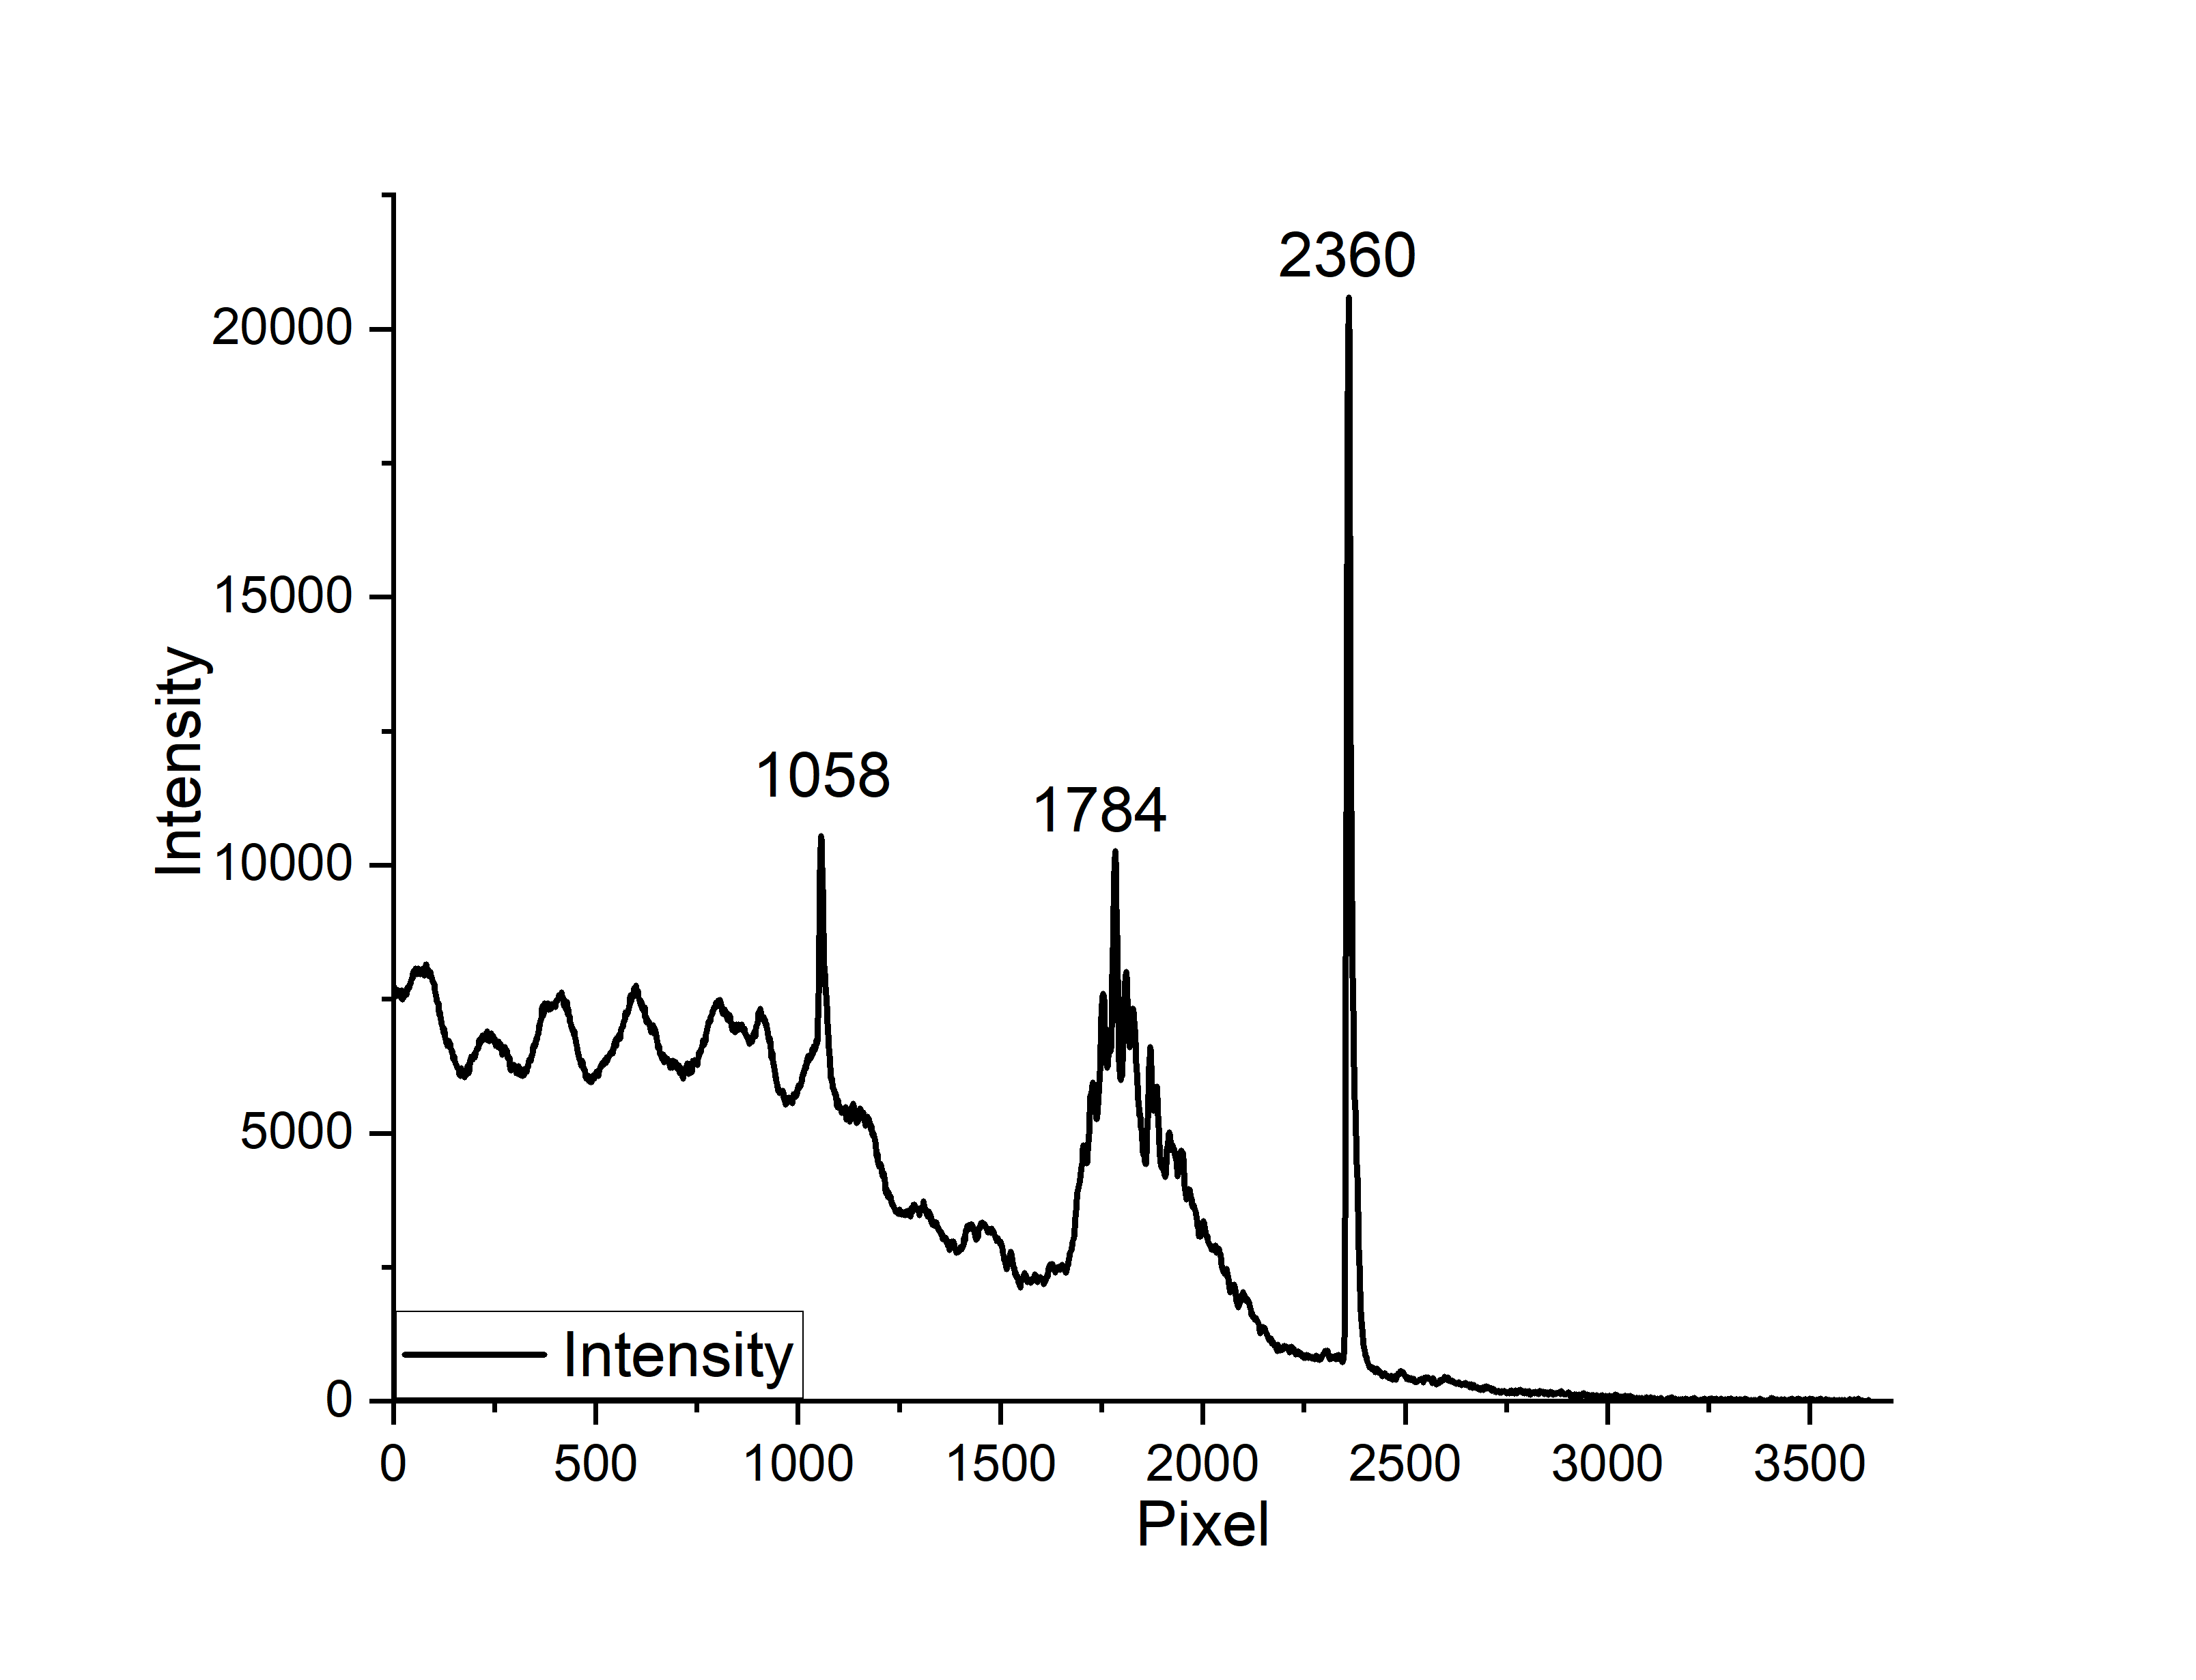
\includegraphics[height = 2.5in,width = 3.2in]{image/biaoding.png}
%        \caption{氘灯标定下的光强-像素图}\label{5--}
%    \end{minipage}
%    %}
%    \centering
%    %\subfigure{
%    \begin{minipage}{0.49\textwidth}
%        \centering
%        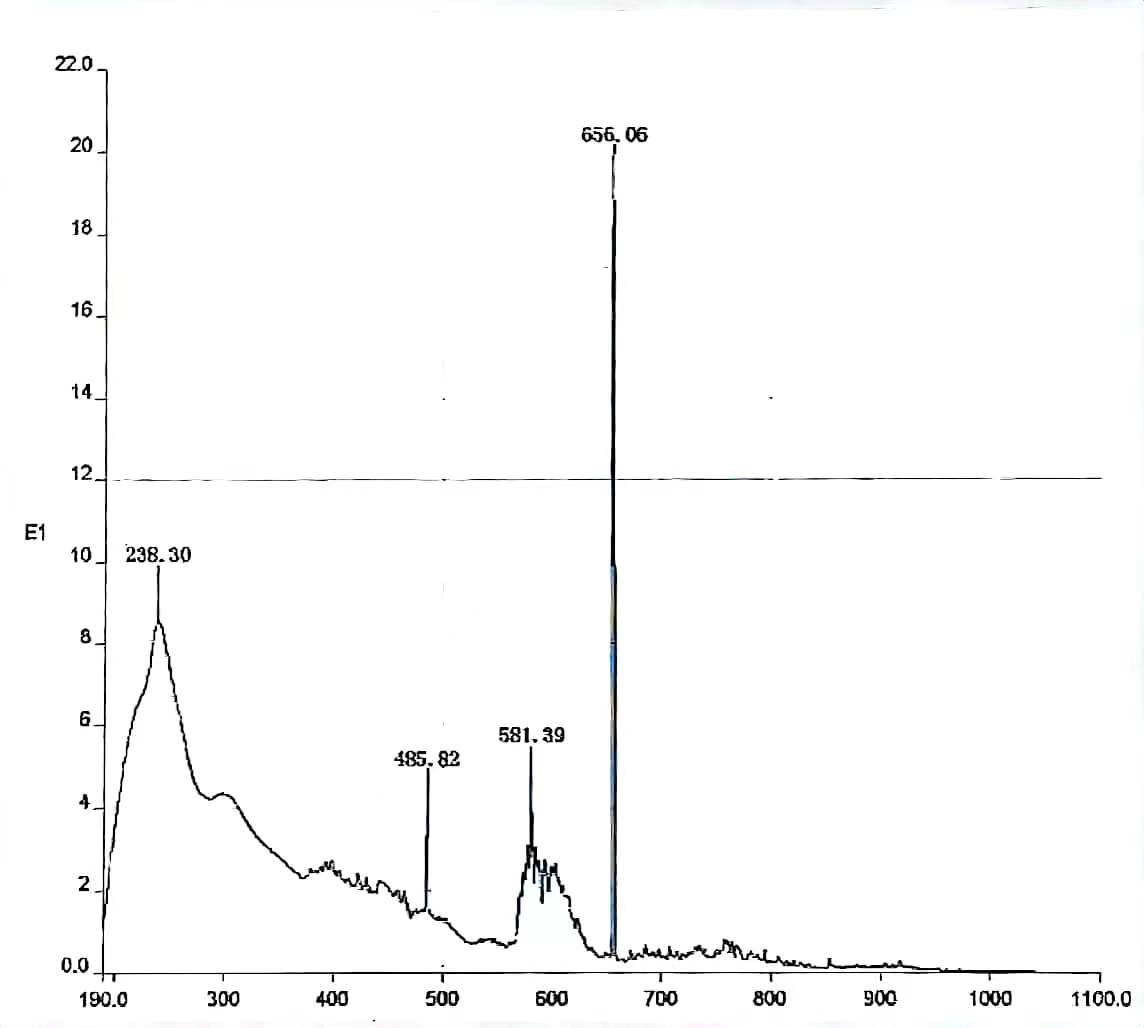
\includegraphics[height = 2.5in,width = 3in]{image/standard.jpg}
%        \caption{氘灯的标准光强-像素图}\label{5-}
%    \end{minipage}
%    %}
%    \centering
%    %\caption{左:氘灯标定下的光强-像素图\quad右:氘灯的标准光强-像素图}\label{5}
%\end{figure}